\chapter{Mean \& Convergence}
\label{ch:meanconv}

Open from \uipth{3.\ Analysis $\to$ Mean \& Convergence}.

The Mean \& Convergence module is the recommended first stop for any new dataset. It serves two purposes: plotting mean velocity profiles along arbitrary lines (similar to the Reynolds stress line-profile mode but for first-order statistics), and quantitatively verifying that the dataset has enough snapshots for the higher-order statistics computed by other modules to be trustworthy.

The module has two tabs: \uipth{Mean Velocity} (line profiles) and \uipth{Convergence} (cumulative statistics at a picked point).

\section{Mean Velocity tab}
\label{sec:meanvel}

This tab plots $\langle U \rangle$, $\langle V \rangle$, and (for stereo data) $\langle W \rangle$ along a user-drawn line, in the same style as Reynolds stress line profiles.

\begin{stepbox}
\begin{enumerate}[leftmargin=1.5em, topsep=2pt]
  \item Choose line orientation: \uipth{Free}, \uipth{Horizontal}, or \uipth{Vertical}.
  \item For Horizontal or Vertical, set \uipth{Spatial avg $\pm$ pts} to average over neighboring rows or columns and reduce noise.
  \item Left-click and drag on the |⟨U⟩| field (left panel) to draw the line.
  \item Click \uipth{Plot Profile}.
\end{enumerate}
\end{stepbox}

\begin{figure}[htbp]
  \centering
  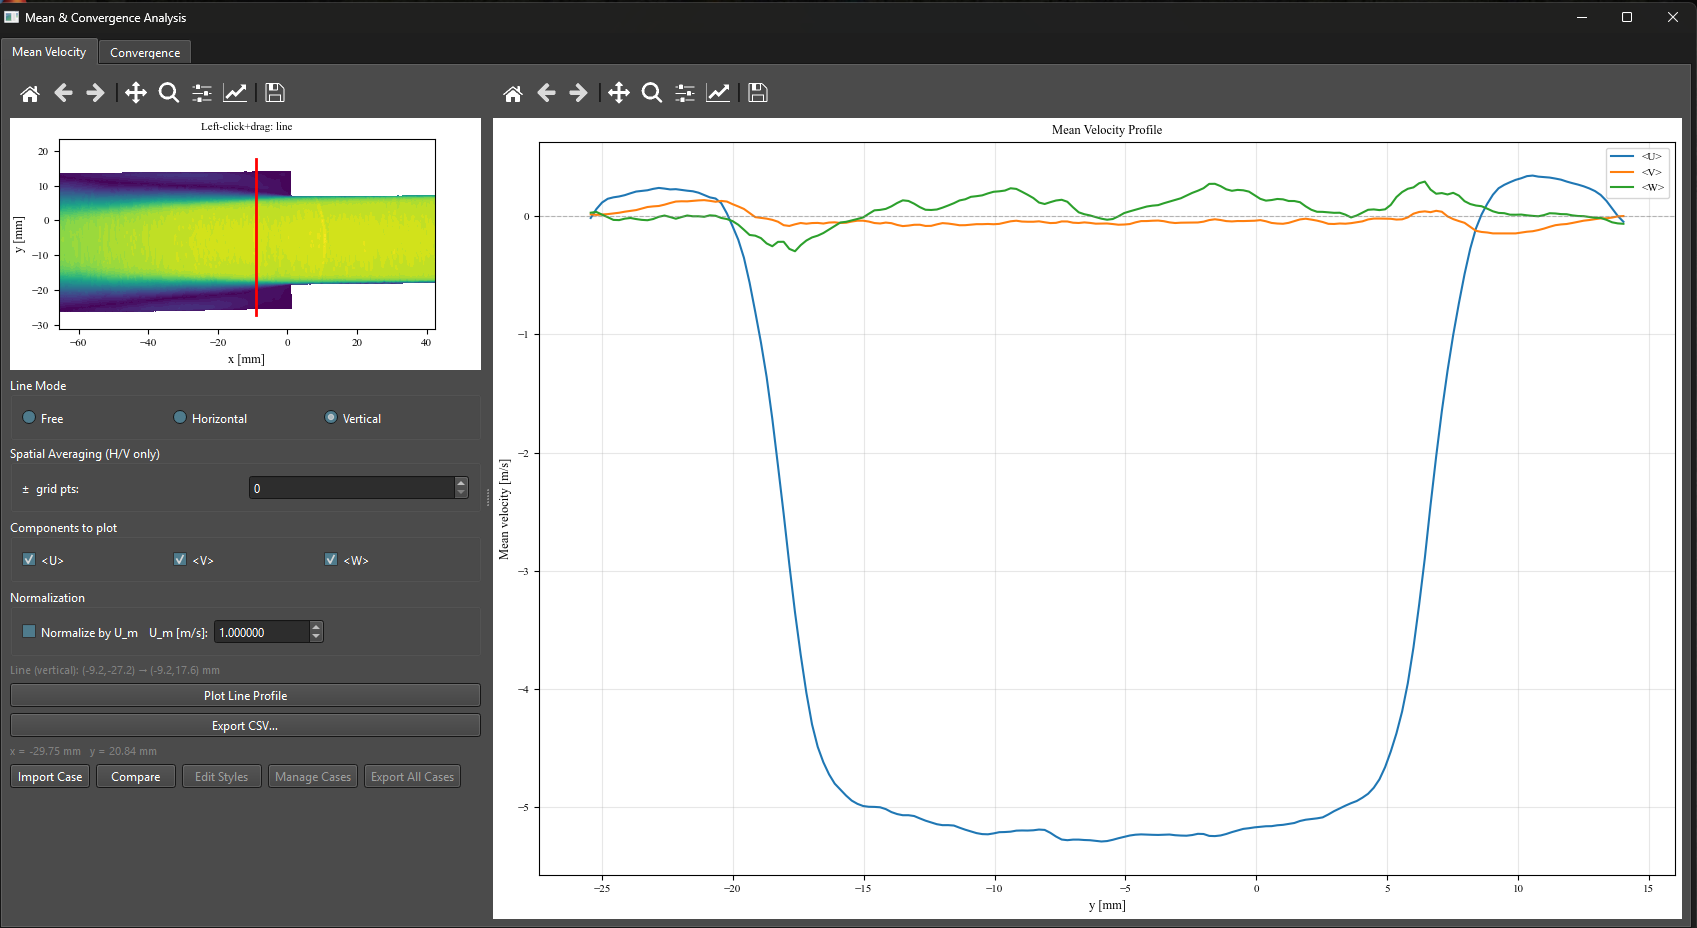
\includegraphics[width=0.92\linewidth]{fig_meanconv_meanvel}
  \caption{Mean \& Convergence module, Mean Velocity tab. Left: $|\langle U \rangle|$ field with a free line drawn (cyan). Right: $\langle U \rangle$, $\langle V \rangle$ profiles along the line as a function of arc length. Stereo data adds $\langle W \rangle$.}
  \label{fig:meanvel}
\end{figure}

\subsection{Normalization by $U_m$}

A checkbox labeled \uipth{Normalize by $U_m$} and a paired spinbox let you divide the plotted velocity components by a user-supplied bulk or reference velocity. When checked, the y-axis labels switch to \texttt{U/U\_m [-]}, \texttt{V/U\_m [-]}, etc. The arc-length axis is not normalized, matching the convention used elsewhere in \software{uPrime}.

\begin{tipbox}
Set $U_m$ to the bulk velocity, free-stream velocity, or any reference value for your flow. Profiles are then directly comparable across cases at different Reynolds numbers.
\end{tipbox}

\subsection{Multi-case comparison}
\label{sec:meanvel_compare}

\software{uPrime} can overlay imported cases (CSV files exported from previous \software{uPrime} sessions or other tools that follow the same column layout) on top of the current profile. This is useful for comparing experimental runs, conditions, or numerical-versus-experimental data.

\begin{stepbox}
\begin{enumerate}[leftmargin=1.5em, topsep=2pt]
  \item Click \uipth{Import Case\ldots} and select a CSV file.
  \item The imported case is added to the case list with an auto-assigned color and dashed linestyle.
  \item Use \uipth{Edit Styles\ldots} to change line color, style, marker, and label per case.
  \item Use \uipth{Manage Cases\ldots} to rename or remove cases.
  \item The current $U_m$ setting is compared against the \texttt{\# U\_m =} header in each imported CSV. If they differ, a status-bar warning is shown for that specific case so you can manually re-normalize before publishing.
\end{enumerate}
\end{stepbox}

The same multi-case workflow is available in Reynolds Stress, TKE Budget, Spectra, Correlation, and Anisotropy windows (see Chapter~\ref{ch:multicase}).

\subsection{Exporting}

Click \uipth{Export Profile\ldots} to save the current profile as a CSV file. The header records the line geometry (endpoints), the $U_m$ value (or N/A if normalization is off), and the column layout. Multi-case overlays can be exported together using \uipth{Export All Cases\ldots}.

\section{Convergence tab}
\label{sec:convergence}

The Convergence tab quantifies whether the dataset has enough snapshots for the first three moments of the velocity fluctuations to be statistically converged. This serves as a numerical check on the assumptions made by every other turbulence-statistics module.

\subsection{Background}

Given a sequence of $N$ snapshots, the cumulative running statistics are
\begin{align}
\langle u' \rangle_N      &= \frac{1}{N} \sum_{i=1}^{N} (u_i - \langle u \rangle_{\mathrm{final}}), \\
\langle u' u' \rangle_N   &= \frac{1}{N} \sum_{i=1}^{N} (u_i - \langle u \rangle_{\mathrm{final}})^2, \\
\langle u' u' u' \rangle_N &= \frac{1}{N} \sum_{i=1}^{N} (u_i - \langle u \rangle_{\mathrm{final}})^3,
\end{align}
where $\langle u \rangle_{\mathrm{final}}$ is the mean computed over all loaded snapshots. With this definition, the curves approach a non-zero asymptote as $N$ grows, which is what allows convergence to be visually inspected.

The cumulative moments are computed using Welford's online algorithm extended to the third central moment. This is a single-pass $O(N)$ computation, numerically stable, and avoids storing per-snapshot residuals.

A trailing-window stability criterion is used to find the convergence point $N^*$:
\[
N^* = \min\left\{ N \;:\; \frac{\max_{n \in [N - W, N]} q_n - \min_{n \in [N - W, N]} q_n}{\sigma_{\mathrm{scale}}} < \varepsilon \right\}
\]
where $W = \max(50, N/10)$ and $\sigma_{\mathrm{scale}}$ is component-aware: $\sqrt{\langle u'u'\rangle_{\mathrm{final}}}$ for first moments, $\langle u'u'\rangle_{\mathrm{final}}$ for second, and $\langle u'u'\rangle_{\mathrm{final}}^{3/2}$ for third (and similarly per-component for $v$ and $w$). The criterion further requires the inequality to hold continuously across the next $W$ samples (sustained crossing), which prevents spurious early matches when the trailing-window range happens to be small by chance.

\noindent\textbf{Reference:} Welford, B.P. (1962). Note on a method for calculating corrected sums of squares and products. \textit{Technometrics}, 4(3), 419--420.

\subsection{Using the tab}

\begin{stepbox}
\begin{enumerate}[leftmargin=1.5em, topsep=2pt]
  \item Set \uipth{Kernel size} (odd integer, default 3). The picked point is averaged over a $k \times k$ neighborhood. Larger kernels reduce noise but cannot pick points within $\lfloor k/2 \rfloor$ of the boundary.
  \item Left-click on the field to pick a point. Points within the boundary margin (shaded grey) are rejected with a status-bar message.
  \item Set the three thresholds: $\varepsilon_1$ for $\langle u' \rangle$, $\varepsilon_2$ for $\langle u'u' \rangle$, $\varepsilon_3$ for $\langle u'u'u' \rangle$. Default 1e-3 each.
  \item Tick which moment orders to plot: $\langle u' \rangle$, $\langle u'u' \rangle$, $\langle u'u'u' \rangle$.
  \item Choose \uipth{Grid layout} (one subplot per component-order combination, raw values) or \uipth{Single plot} (all selected curves overlaid, normalized).
  \item Click \uipth{Compute Convergence}.
\end{enumerate}
\end{stepbox}

\begin{figure}[htbp]
  \centering
  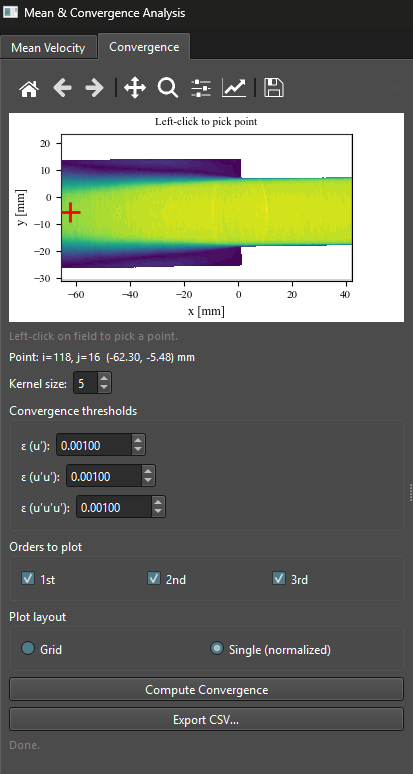
\includegraphics[width=0.6\linewidth]{fig_meanconv_picker}
  \caption{Convergence tab, point picker. The $|\langle U \rangle|$ field is shown in viridis. The boundary margin (grey overlay) is determined by the kernel size and clicks inside it are rejected. The picked point and kernel footprint are shown as a red marker.}
  \label{fig:convpicker}
\end{figure}

\subsection{Grid layout (raw values)}

In grid mode, $\langle u' \rangle_N$, $\langle u'u' \rangle_N$, and $\langle u'u'u' \rangle_N$ are plotted in physical units, one subplot per component (rows: $u$, $v$, optionally $w$) and per moment order (columns: 1, 2, 3). A pair of dashed horizontal lines marks the threshold band $q_{\mathrm{final}} \pm \varepsilon \cdot \sigma_{\mathrm{scale}}$ around the asymptote, and a vertical line at $N^*$ shows the sustained-crossing convergence point. Curves that never satisfy the criterion are labeled \uipth{Not converged}.

\begin{figure}[htbp]
  \centering
  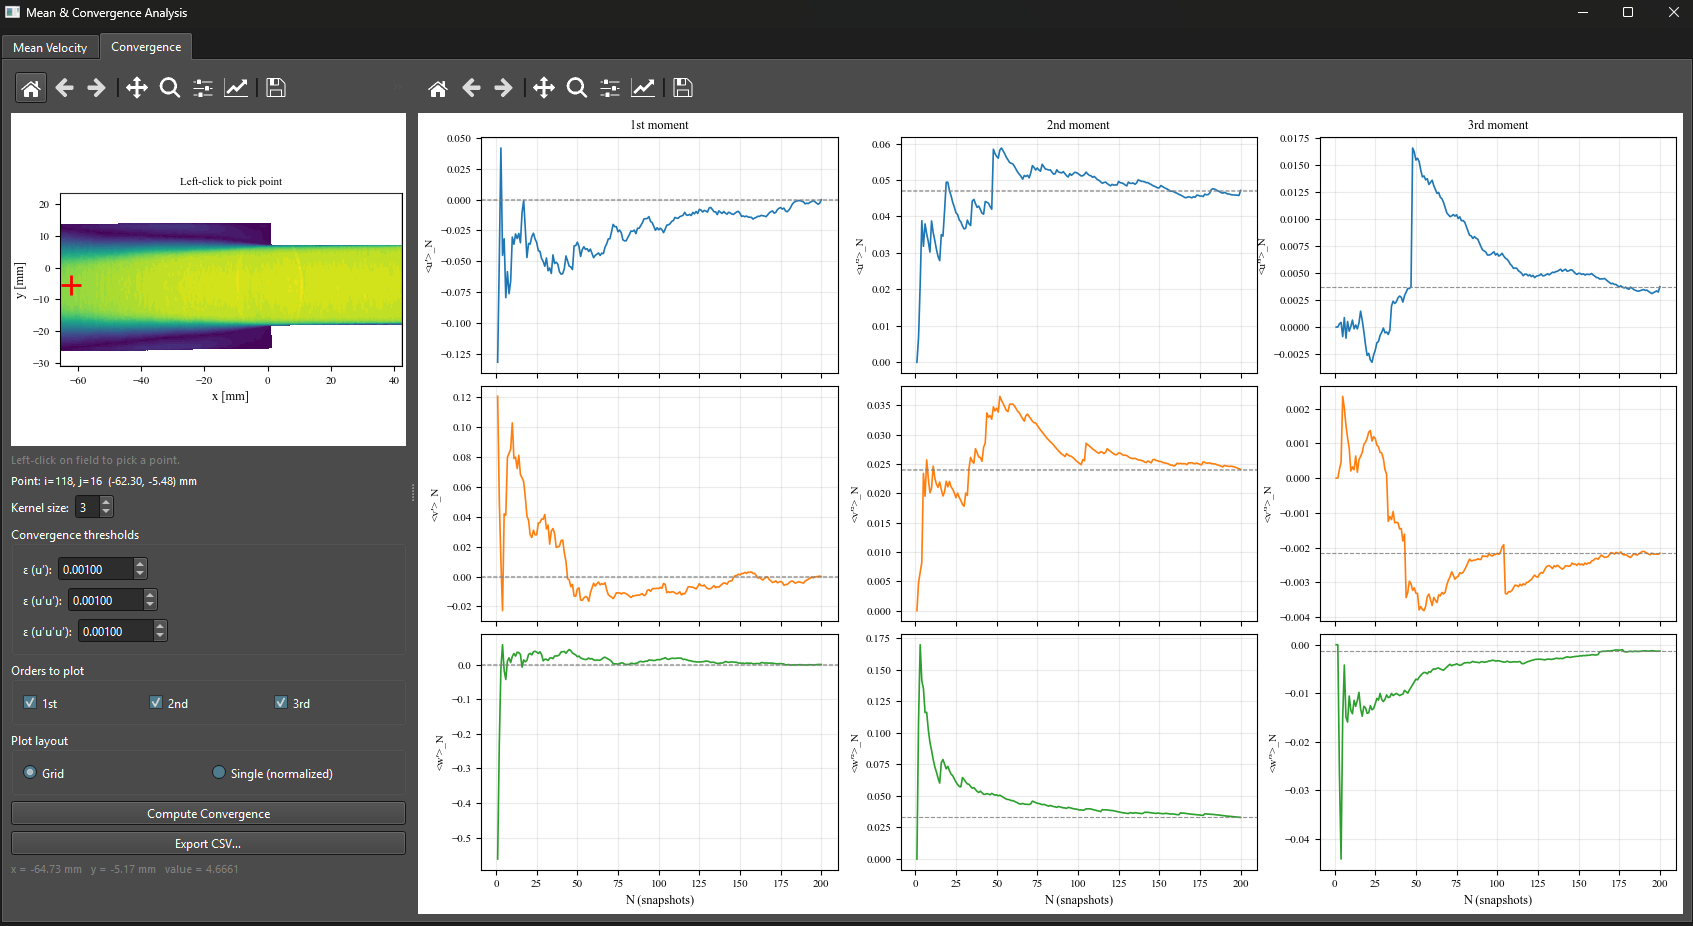
\includegraphics[width=0.92\linewidth]{fig_meanconv_grid}
  \caption{Convergence tab, grid layout (planar 2D2C: $2 \times 3$ subplots). Each panel shows a cumulative moment in physical units, the dashed threshold band around its final-value asymptote, and the vertical $N^*$ line where the sustained-crossing criterion is first met. Third moments typically require many more snapshots than first or second moments to converge.}
  \label{fig:convgrid}
\end{figure}

\subsection{Single plot (normalized)}

In single-plot mode, every selected curve is normalized by its own scale $\sigma_{\mathrm{scale}}$ so they share a common dimensionless y-axis. Curves are color-coded by component ($u$, $v$, $w$) and styled by moment order (solid for first, dashed for second, dotted for third). Per-component dashed threshold bands are drawn around each curve's asymptote $q_{\mathrm{final}}/\sigma_{\mathrm{scale}}$.

\begin{figure}[htbp]
  \centering
  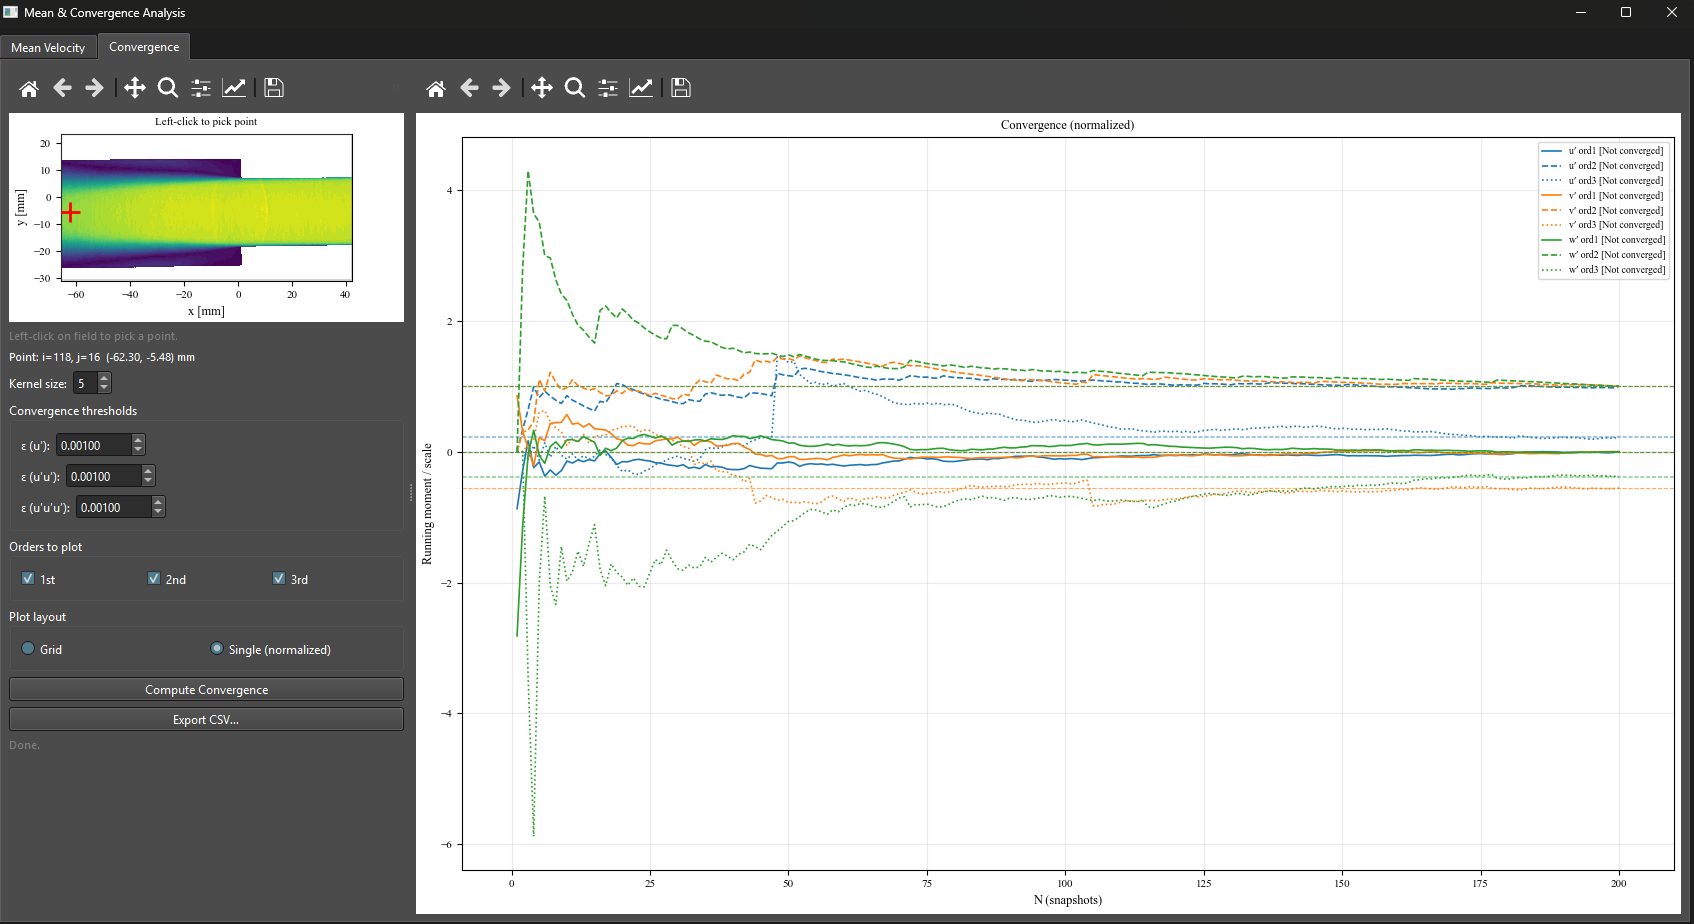
\includegraphics[width=0.92\linewidth]{fig_meanconv_single}
  \caption{Convergence tab, single normalized layout. All selected curves are overlaid on one axes and approach their respective non-zero asymptotes (one per curve). Per-component dashed threshold bands flank each asymptote.}
  \label{fig:convsingle}
\end{figure}

\subsection{Exporting}

Click \uipth{Export CSV\ldots} to save the cumulative moments. The header block records the picked point indices and physical coordinates, the kernel size, the three thresholds, the dataset $N_{\mathrm{total}}$, and the $N^*$ value computed for each quantity. The columns are $N$, $\langle u' \rangle_N$, $\langle u'u' \rangle_N$, $\langle u'u'u' \rangle_N$, $\langle v' \rangle_N$, ..., adding $w$ components for stereo data.

\begin{tipbox}
First and second moments typically converge with a few hundred snapshots in well-mixed regions. Third moments often require 5000 or more, and may not converge at all in regions of low intensity. A non-converging $\langle u'u'u' \rangle$ is not necessarily a problem for second-order statistics; the convergence module simply makes this explicit.
\end{tipbox}

\section{Inline non-convergence notice}
\label{sec:convnotice}

The Reynolds Stress, TKE Budget, and Spectral Analysis windows display a persistent amber top-bar label when the loaded dataset has fewer than 500 snapshots:

\begin{center}
\fcolorbox{upaccent!60}{red!5}{\parbox{0.85\linewidth}{\centering \small \faExclamationTriangle\quad Only \textbf{N=234} snapshots loaded. Statistics may not be converged. Use the Mean \& Convergence module to verify.}}
\end{center}

The label is hidden automatically when the dataset has 500 or more snapshots. Other modules (Correlation, Anisotropy, POD, DMD, Vortex Identification) are silent. The 500 threshold is hardcoded in \texttt{core/constants.py} as \texttt{CONVERGENCE\_WARNING\_N} and can be changed in source builds.

\begin{figure}[htbp]
  \centering
  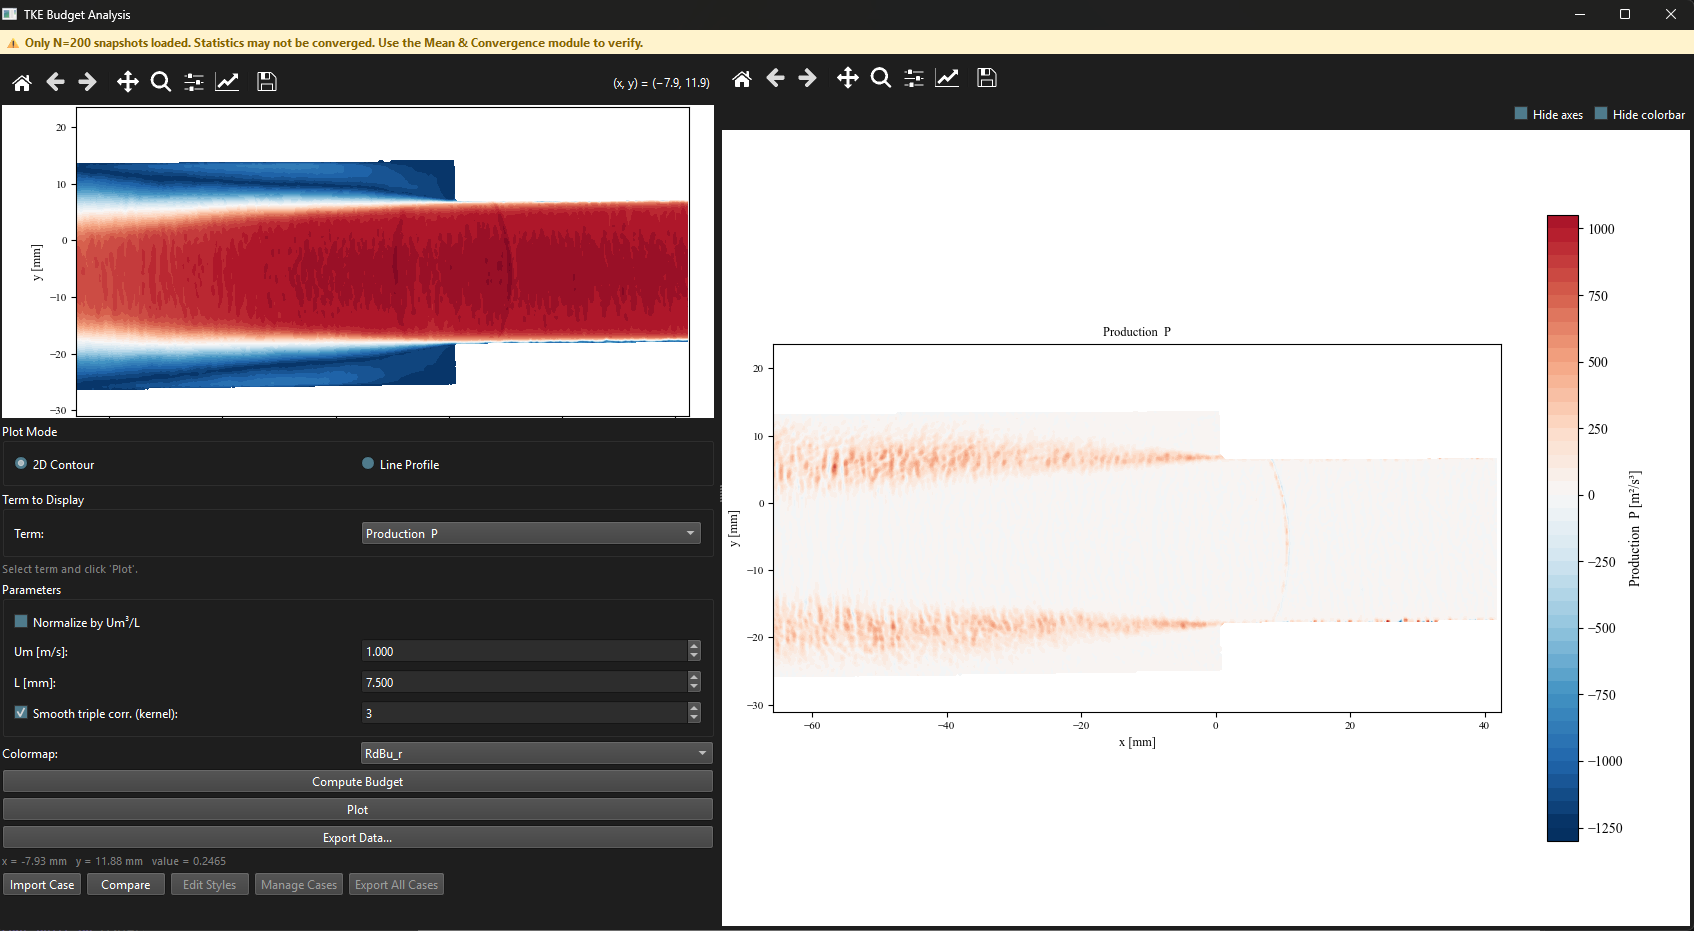
\includegraphics[width=0.85\linewidth]{fig_convergence_topbar}
  \caption{Top-bar non-convergence label as it appears in the Reynolds Stress window with $N = 234$ snapshots. The label is hidden automatically once $N \geq 500$.}
  \label{fig:convbar}
\end{figure}

% ============================= CHAPTER 5 ==============================
